\documentclass[tikz,border=6pt]{standalone}
\usepackage{pgfplots}
\pgfplotsset{compat=1.18}
\begin{document}
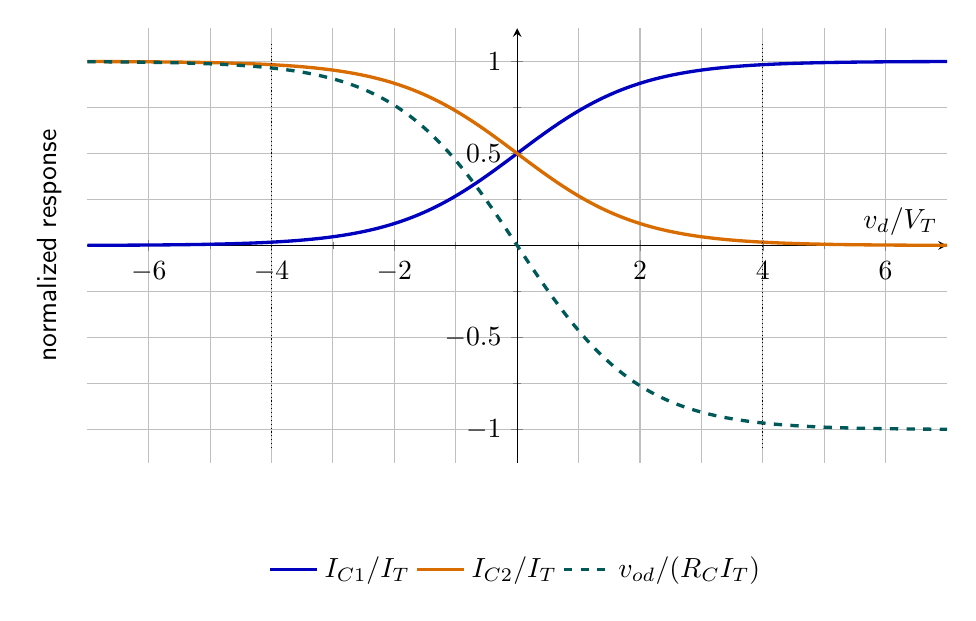
\begin{tikzpicture}[font=\sffamily]
\begin{axis}[
 width=12.5cm,height=7.1cm,
 axis lines=middle,xlabel={$v_d/V_T$},ylabel={normalized response},
 ylabel style={at={(axis description cs:-.07,.5)},rotate=90},
 xmin=-7,xmax=7,ymin=-1.18,ymax=1.18,
 xtick={-6,-4,-2,0,2,4,6},ytick={-1,-.5,0,.5,1},
 grid=both,minor tick num=1,
 legend style={at={(0.5,-0.19)},anchor=north,legend columns=3,draw=none}]
 \addplot[blue!75!black,very thick,domain=-7:7,samples=180]
   {1/(1+exp(-x))};
 \addlegendentry{$I_{C1}/I_T$}
 \addplot[orange!85!black,very thick,domain=-7:7,samples=180]
   {1/(1+exp(x))};
 \addlegendentry{$I_{C2}/I_T$}
 \addplot[teal!70!black,very thick,dashed,domain=-7:7,samples=180]
   {-tanh(x/2)};
 \addlegendentry{$v_{od}/(R_CI_T)$}
 \draw[densely dotted] (axis cs:-4,-1.1) -- (axis cs:-4,1.1);
 \draw[densely dotted] (axis cs:4,-1.1) -- (axis cs:4,1.1);
\end{axis}
\end{tikzpicture}
\end{document}
